\subsection{RQ3: How much interference is visible in one heterogeneous pair?}
The RTX 5070 Ti averages 73.01$\pm$1.41 tok/s alone and 72.36$\pm$2.26 tok/s while an RTX 5060 Ti x4 simultaneously runs at 59.14$\pm$1.24 tok/s lane-local TG (Figure~\ref{fig:hetero}). Using the eight run means per arm, the unadjusted concurrent-minus-solo change is $-0.65$ tok/s ($-0.9\%$); Welch's test gives $p=0.50$ and a 95\% CI of $[-2.71,+1.41]$ tok/s. The raw TG variation is strongly associated with per-run speculative acceptance (Pearson $r=0.93$ solo and $r=0.95$ concurrent). In an exploratory OLS model, $TG\sim\mathrm{concurrent}+\mathrm{acceptance}$, the concurrent coefficient is $-1.00$ tok/s (about $-1.4\%$, 95\% CI $[-1.71,-0.30]$, $p=0.009$), with residual SD 0.65 tok/s. Because speculative acceptance is measured during execution and may itself respond to concurrency, we report this as a sensitivity analysis rather than a causal estimate. The unadjusted estimate is inconclusive; the acceptance-adjusted model indicates a small shared-resource cost in this measured pair.

\begin{figure}[t]
\centering
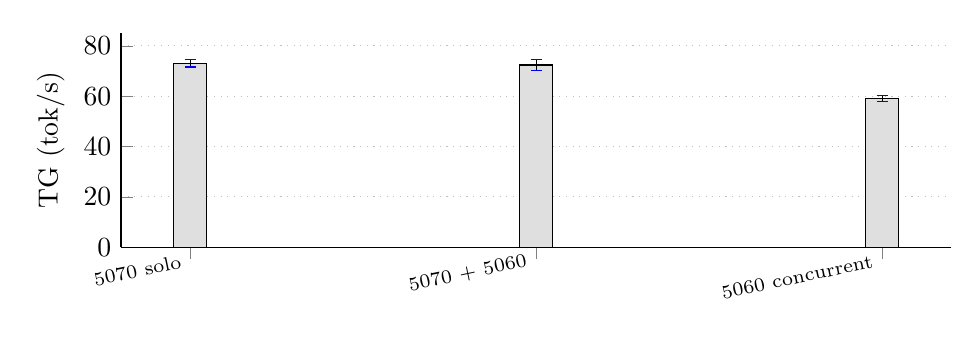
\begin{tikzpicture}
\begin{axis}[
width=\columnwidth,height=4.3cm,
ybar,bar width=12pt,ymin=0,ymax=85,
xtick=data,xticklabels={5070 solo,5070 + 5060,5060 concurrent},
xticklabel style={font=\scriptsize,rotate=12,anchor=east},
ylabel={TG (tok/s)},axis lines*=left,ymajorgrids=true,major grid style={dotted},
error bars/y dir=both,error bars/y explicit,
]
\addplot+[draw=black,fill=gray!25,error bars/y dir=both,error bars/y explicit]
coordinates {(1,73.01) +- (0,1.41) (2,72.36) +- (0,2.26) (3,59.14) +- (0,1.24)};
\end{axis}
\end{tikzpicture}
\caption{Same-generation heterogeneous concurrency (mean $\pm$ SD, $n=8$ fast-lane runs per arm). Raw means differ by $-0.9\%$; an exploratory acceptance-adjusted OLS model estimates $-1.4\%$ (95\% CI $-2.3$ to $-0.4\%$).}
\label{fig:hetero}
\end{figure}

This experiment is evidence about interference within the independent-lane design, not a comparison against coupled execution. The two concurrent lane-local TG means sum to 131.5 tok/s, but these rates must not be treated as common-wall throughput. The retained concurrent requests complete at a common-wall aggregate of 116.96$\pm$2.42 tok/s because the wall interval extends until the slower request finishes. Thus the slower lane adds useful capacity while imposing a small measurable shared-resource cost on the fast lane; it does not make the two lane-local rates directly additive under a fixed-length makespan metric. The scope is limited: both GPUs are same-generation Blackwell cards with 16~GB VRAM, and GPU model and PCIe width change together.

\subsection{RQ4: How workload-dependent are PP and TG?}
